\label{sec:xadd}

In this section, we describe the case representation of symbolic functions and how decision diagrams data structures can be used to store and manipulate them.

\subsection{CASE REPRESENTATION}

We are interested in the symbolic representation of piecewise polynomial functions defined over discrete and continuous domains. Given a set of boolean and continuous variables $(\vec{b},\vec{x}) = ( b_1,\ldots,b_n,x_{1},\ldots,x_m )$, where $b_i \in \{ 0,1 \}$ ($1 \leq i \leq n$) and $x_j \in \mathbb{R}$ ($1 \leq j \leq m$), we will represent symbolic piecewise polynomials in \emph{case} form~\cite{fomdp}:
{%\footnotesize 
\begin{align}
f(\vec{b},\vec{x}) = 
\begin{cases}
  \phi_1(\vec{b},\vec{x}): & f_1(\vec{x}) \\ 
 \vdots&\vdots\\ 
  \phi_k(\vec{b},\vec{x}): & f_k(\vec{x}) \\ 
\end{cases} \label{eq:case}
\end{align}
}
Here the $f_i$ are polynomial functions over the continuous variables $\vec{x}$ and the $\phi_i$ are logical formulae defined over the state $(\vec{b},\vec{x})$ that can include arbitrary logical ($\land,\lor,\neg$) combinations of (i) boolean variables and (ii)  strict\footnote{ For purposes of evaluating a linear function $f$ within a region, it does not matter whether a bound is inclusive ($\leq$ or $\geq$) or exclusive ($<$ or $>$), since it can be arbitrarily near the bounds; for precise evaluation at the bounds, $f$ is required to be continuous, in which case both partitions will give the same result.} inequalities ($>,<$) comparing polynomial expressions over the continuous variables  over continuous variables.  

The $\phi_i$ are required to be disjoint from each other;  however they may not exhaustively cover the state space, in which case $f$ is a \emph{partial function}, undefined for some variable assignments. Since they represent parts of the piecewise function, pairs $(f_i,\phi_i)$ are referred to as cases or partitions of $f$, moreover, these are identified with a piecewise function of a single partition, which is called a case function.

We are specially interested in piecewise linear functions and case linear functions, in which case all $f_i$ and all expressions in the inequalities in $\phi_i$ are linear. In this case, we note that any logical formula can be rewritten as a disjunction of conjunctive formulas, so that we can write $\phi_i$ = $\bigvee_{j=0}^{n_i} \theta_{ij}$ where each $\theta_{ij}$ is a conjunction of boolean variables and  linear inequalities, and $n_i$ is the number of conjunctive formulas obtained from $\phi_i$. As $\theta_{ij}$ is only conjunctive, there is a partial boolean assignment necessary for $\theta_{ij}$ to be satisfied, denoted $\vec{b}_{\theta_{ij}}$ and the conjunction of the linear inequalities in $\theta_{ij}$ define a convex feasible region in $\mathbb{R}^m$, denominated the polytope of $\theta_{ij}$ and denoted $Polyt(\theta_{ij})$. We observe that the inequalities in $\theta_{ij}$ may define unfeasible or unbounded regions, but we discard unfeasible combinations and add special minimal and maximal bounds for every continuous variable so that all polytopes considered are feasible and bounded. This regions are important when evaluating the image of $f$, because $f$ takes the value of $f_i$ in a constrained region $C(\phi_i)$, that is the union of polytopes from $\phi_i$.
		$$C(\phi_i) = \bigcup_j Polyt(\theta_{ij})$$

TODO: Make picture to examplify $f$, $f_i$, $\phi$, $\theta$, a polytope and a region $C_i$...

\begin{figure}[h!t]
\center
\fbox{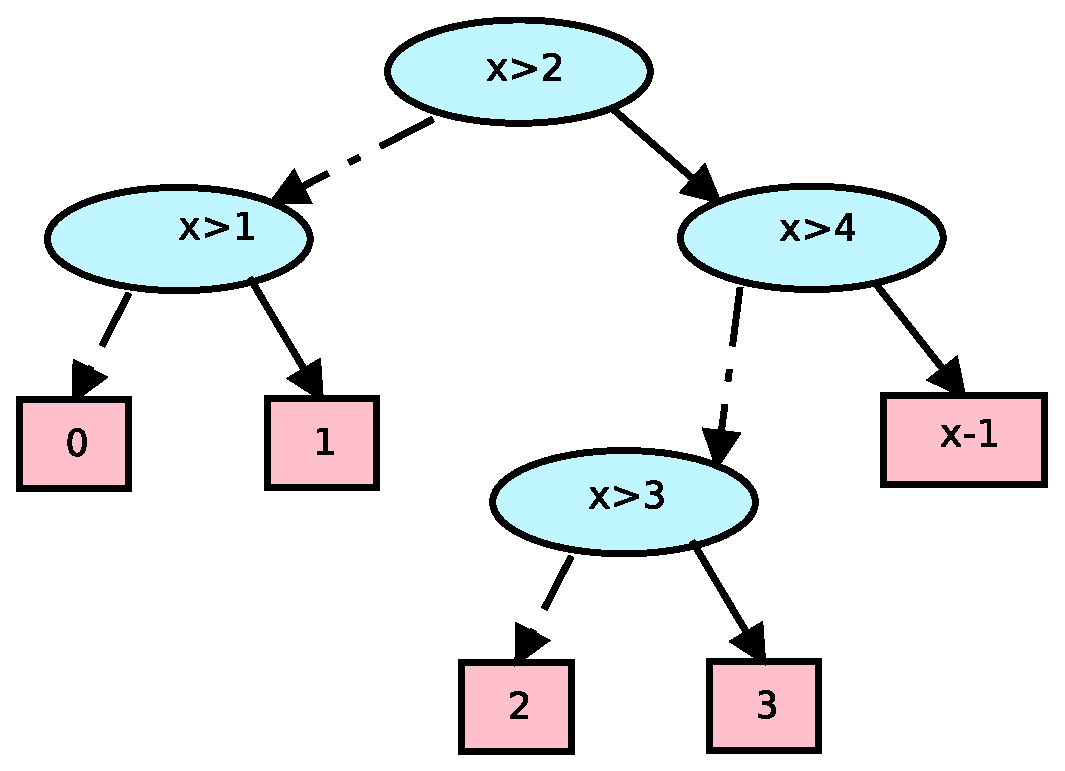
\includegraphics[scale=0.4]{Figures/xadds/samplexadd.eps} }
\caption{ Example of symbolic function in case form, graph showing the continuous domain for each partition.}
\label{fig:samplecase} 
\end{figure}

%Now we define the basic operations that can be performed on symbolic functions in case representationIn the context of SDP, we need to perform operations on symbolic functions represented in case form. The operations we need are: scalar multiplication, addition, subtraction and multiplication of symbolic functions, case maximization, boolean restriction and continuous integration. This operations were a major contribution of \cite{sanner_uai11} and we refer to that for the detailed definitions. 

%%%%%%%%%%%%%%%%%%%%%%%%%%%%%%%%%%%%%%%%%%%%%%%%%%%%%%%%%%%%%%%%%%%%%%%%
%\incmargin{.5em}
%\linesnumbered
%\begin{algorithm}[th!]
%\vspace{-.5mm}
%\dontprintsemicolon
%\SetKwFunction{regress}{Regress}
%\SetKwFunction{approximate}{Approximate}
%\Begin{
%   $V^0:=0, h:=0$\;
%   \While{$h < H$}{
%       $h:=h+1$\;
%       \ForEach {$a(\vec{y}) \in A$}{
%              $Q_a^{h}(\vec{y})\,:=\,$\regress{$V^{h-1},a,\vec{y}$}\;
%              $Q_a^{h} := \max_{\vec{y}} \, Q_a^{h}(\vec{y})$ $\,$ \emph{// Continuous $\max$}\;
%              $V^{h} := \casemax_a \, Q_a^{h}$ $\,$ \emph{// $\casemax$ all $Q_a$}\;
%              $\pi^{*,h} := \argmax_{(a,\vec{y})} \, Q_a^{h}(\vec{y})$\;
%       }
%       $V^h = $\approximate{$V^{h}$}\; \label{approxline}
%       \If{$V^h = V^{h-1}$}
%           {break $\,$ \emph{// Terminate if early convergence}\;}
%   }
%     \Return{$(V^h,\pi^{*,h})$} \;
%}
%\caption{\footnotesize \texttt{VI}(Hybrid-MDP, $H$) $\longrightarrow$ $(V^h,\pi^{*,h})$ \label{alg:vi}}
%\vspace{-1mm}
%\end{algorithm}
%\decmargin{.5em}
%%%%%%%%%%%%%%%%%%%%%%%%%%%%%%%%%%%%%%%%%%%%%%%%%%%%%%%%%%%%%%%%%

\begin{comment}
Next we define the basic operations that can be applied on symbolic functions:

\emph{Unary operations} such as scalar multiplication $c\cdot f$ (for $c \in \mathbb{R}$) is simply applied to each $f_i$ ($1 \leq i \leq k$). Intuitively, to perform a \emph{binary
  operation} on two case statements, we simply take the cross-product
of the logical partitions of each case statement and perform the
corresponding operation on the resulting paired partitions. For instance, we define perform sum($\oplus$), subtraction($\ominus$) and product($\otimes$) by,
respectively, adding, subtracting or multiplying partition values to obtain the result. 

Next we define \emph{symbolic case maximization}:
{\footnotesize
\begin{center}
\begin{tabular}{r c c c l}
&
\hspace{0mm} $\casemax \Bigg(
  \begin{cases}
    \phi_1: \hspace{-2mm} & \hspace{-1mm} f_1 \\ 
    \phi_2: \hspace{-2mm} & \hspace{-1mm} f_2 \\ 
  \end{cases}$
$,$
&
\hspace{0mm}
  $\begin{cases}
    \psi_1: \hspace{-2mm} & \hspace{-1mm} g_1 \\ 
    \psi_2: \hspace{-2mm} & \hspace{-1mm} g_2 \\ 
  \end{cases} \Bigg)$
&
\hspace{0mm} 
$ = $
&
\hspace{0mm}
  $\begin{cases}
  \phi_1 \wedge \psi_1 \wedge f_1 > g_1    : & \hspace{-2mm} f_1 \\ 
  \phi_1 \wedge \psi_1 \wedge f_1 \leq g_1 : & \hspace{-2mm} g_1 \\ 
  \phi_1 \wedge \psi_2 \wedge f_1 > g_2    : & \hspace{-2mm}f_1 \\ 
  \phi_1 \wedge \psi_2 \wedge f_1 \leq g_2 : & \hspace{-2mm} g_2 \\ 
  \hspace{1cm}\vdots \hspace{8mm}: & \hspace{-2mm} \vdots
  \end{cases}$
\end{tabular}
\end{center}
} If all $f_i$ and $g_i$ are linear,
the $\casemax$ result is clearly still linear and representable in the case format previously described (i.e., linear inequalities in decisions). As linear inequalities can be inconsistent (infeasible) some of the generated partitions will be removed from the result. 

 The operation of \emph{boolean restriction} required for regressing boolean variables is obvious and an example is omitted: in this operation
$f|_{b=v}$, anywhere a boolean variable $b$ occurs in $f$, we assign
it the value $v \in \{ 0,1 \}$, and resolve the following logic implications, reducing formulae or removing partitions.  The operation of \emph{continuous integration} $\int Q(x'_j) \otimes P(x'_j|\cdots) dx'_j$ is required for regressing continuous variables. As previously defined, $P(x_j'|\cdots)$ will always be of the form $\delta[x_j' - h(\vec{z})]$ where
$h(\vec{z})$ is a case statement and $\vec{z}$ does not contain
$x'_j$.  Rules of integration then tell us that $\int f(x'_j) \otimes
\delta[x_j' - h(\vec{z})] dx'_j = f(x'_j) \{ x'_j / h(\vec{z}) \}$
where the latter operation indicates that any occurrence of $x'_j$ in
$f(x'_j)$ is \emph{symbolically substituted} with the case statement
$h(\vec{z})$. The appearance of case statement within formulae is solved expanding the cross-product of the logical partitions. A more detailed specification of this operation is available in ~\cite{sanner_uai11}.  The important insight is that this $\int$ operation yields a result that is a
case statement in the form previously outlined.

The only operation for SDP that has not yet been defined is the continuous action maximization.
The continuos maximization over action variables can be wrtitten as $g(\vec{b},\vec{x}) := \max_{\vec{y}} \, f(\vec{b},\vec{x},\vec{y})$. Note that the result of this max, $g(\vec{b},\vec{x})$ is a function of continuous variables, hence requiring \emph{symbolic} constrained optimization.

The definition of this maximization operation was the major contribution of~\cite{zamani12}, so refer to this work for a detailed explanation. We outline the basic steps for continuous maximization.

First, due to the commutativity of $\max$, any multivariate $\max_{\vec{y}}$ can be rewritten as a sequence of univariate $\max$ operations $\max_{y_1} \cdots \max_{y_{|\vec{y}|}}$; hence it
suffices to provide just the \emph{univariate} $\max_y$ solution:
$g(\vec{v}) := \max_{y} \, f(\vec{v},y)$, where $\vec{v}$ denotes a vector of boolean and continuous variables, in our case containing $\vec{b}$, $\vec{x}$ and other action parameters.

Second, because of the mutual disjointness of partitions, and the commutativity of $\casemax_i$ and $\max_y$, we can write $\max_y f(\vec{v},y) $ via:
{\footnotesize
\begin{align}
\max_y f(\vec{v},y) & = 
\max_y \casemax_i \, \phi_i(\vec{v},y) f_i(\vec{v},y) \nonumber \\
& = \casemax_i \, \fbox{$\max_y \phi_i(\vec{v},y) f_i(\vec{v},y)$} \label{eq:casemax_max}
\end{align}}

 Thus to complete this operation we need only
show how to symbolically compute the maximum in a single partition 
$\max_y \phi_i(\vec{v},y) f_i(\vec{v},y)$.

%In $\phi_i$, we observe that each conjoined constraint serves one of
%three purposes: (i) \emph{upper bound on $y$}: it can be written
%as $y < l(\vec{v})$; (ii) \emph{lower bound on $y$}: it can be written as $y >
%u(\vec{v})$ or (iii) \emph{independent of $y$}: the constraints do not contain $y$
%and can be safely factored outside of the $\max_y$, as $f_i(\vec{v},y) =  g_i(\vec{v})$.  
%Because there are multiple symbolic upper and lower
%bounds on $y$, we apply the $\casemax$ ($\casemin$) operator to determine the highest lower bound (lowest upper bound):

%The substitution operator $\{ y / f \}$ replaces $y$ with case statement $f$, 
%defined in~\cite{sanner_uai11}.

\end{comment}









\subsection {\bf DECISION DIAGRAMS}
Here we introduce the XADD data structure that provides a compact way to support case statements and symbolic piecewise polynomials. As it is an extension, we begin by defining the simpler form, the Algebraic Decision Diagrams(ADD).

\subsubsection{Algebraic Decision Diagrams(ADDs)} 

ADDs~\cite{bahar93add}, provide a compact way to represent and perform operations on functions from boolean vector domains to a real-value range ( $\{ 0, 1\}^n \rightarrow \mathbb{R}$). 

An ADD represents these functions as a directed acyclic graph(DAG), where, similar to a decision tree, each internal node is associated to one of the boolean variables, and it has two outward edges, the high($h$) and low($l$) that are chosen when the boolean variable is assigned to respectively $1$ or $0$. The difference between an ADD and a decision tree is in the possibility of convergent paths, as two internal nodes may share a descendent, which can greatly increase compactness. The terminal nodes contain a real value, which is the value of the represented function for all boolean assignments that reach this terminal node when evaluated in the DAG.

 Also, for efficient execution of operations between ADDs, it is required that they share a variable ordering, which produces a canonical diagram, unique for each function~\ref{canonADD}. ||TODO: Reference for ADD canonicity|| ADDs produce efficient representation of functions with context-specific independence and redundant structure. For example, functions of the form $\sum_{i=0}^k b_i$ would produce decision trees with an exponential number of nodes, while the ADD representation is quadratic on $k$. Operations that can be efficiently performed in ADDs include unary operation such as min, max and marginalization over variables, as well as binary operations such as addition, subtraction, multiplication, division, min and max.

One additional feature of ADDs, is that there exists an efficient bounded error approximation algorithm~\cite{apricodd}. It works by collecting and merging all similar valued leaves incurring less error than an specified tolerance. As this causes some internal nodes to be redundant they are removed, and the ADD size and height may be reduced. An example of the ADD approximation is provided in figure \ref{fig:addapprox}.

\begin{figure}[h!t]
\center
\fbox{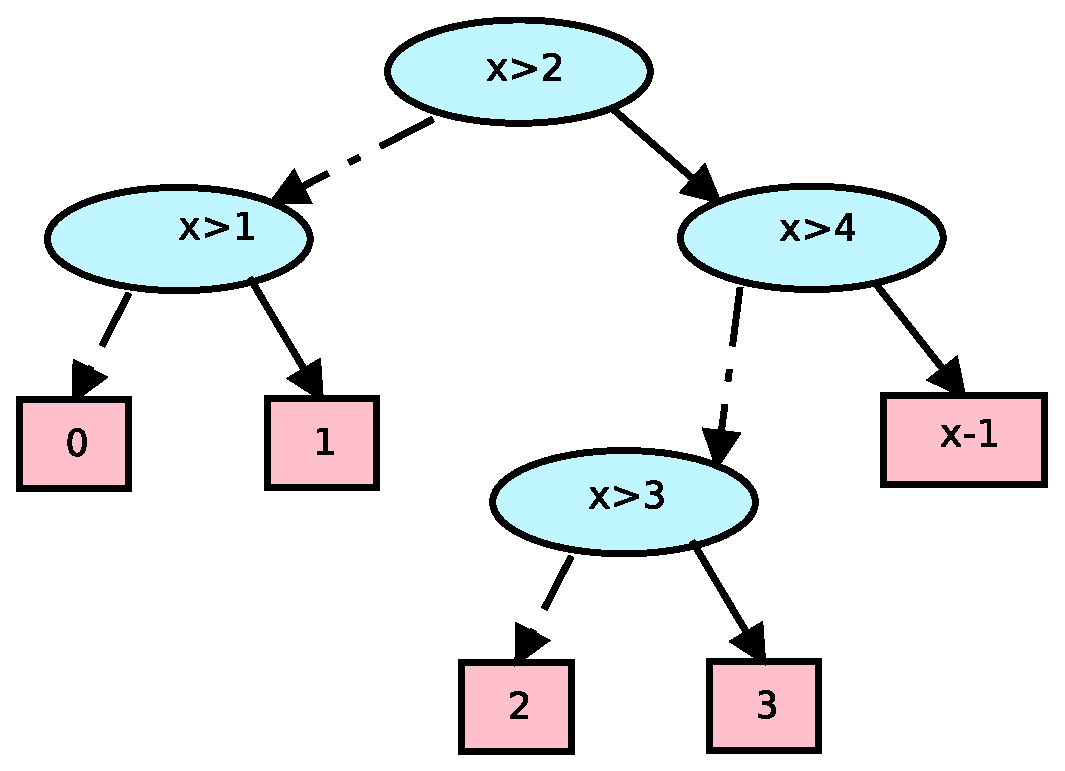
\includegraphics[scale=0.4]{Figures/xadds/samplexadd.eps} }
\caption{ Example of ADD.}
\label{fig:addapprox} 
\end{figure}


\subsubsection{Extended Algebraic Decision Diagrams(XADDs)} 

The XADD~\cite{sanner_uai11} data structure is an extension of ADD, that allows greater expressivity, representing symbolic piecewise polynomials. More specifically, the functions that are represented in a XADD are of the form $f : \{ 0, 1\}^n\times \mathbb{R}^m \rightarrow \mathbb{E}(\mathbb{R}^m)$, where $\mathbb{E}(\mathbb{R}^m)$ denotes the set of expressions containing real-valued constants and the continuous variables related by operations of addition or multiplication.

Here is the formal definition of XADDs as a BNF grammar:

$<$Node$>$ $=$ Internal $|$ Terminal.\\
$<$Terminal$>$ $=$ TermExpr.\\
$<$Expr$>$ $=$ Term $|$ Term "+" Expr.\\
$<$Term$>$ $=$ $c \prod_{i=1}^m {x_i^{\alpha_i }}$.\\
$<$Internal$>$ $=$ Decision "?" highNode  ":" lowNode.\\
$<$Decision$>$ $=$ $b_k$ $|$ Ineq.\\
$<$Ineq$>$ $=$ IneqExpr "$>$" 0.\\

Here, $b_k$ is a boolean variable, and $x_i$ are the continuous variables in this XADD. $c$ is a real number, $\alpha_i$ are positive integers, highNode and lowNode are elements of the Node grammar and TermExpr and IneqExpr are elements of the Expr grammar.
For the case of linear XADDs, the generation rule for continuous expressions is simplified: $<$Expr$>$ $=$ $\vec{c}\cdot\vec{x_0}$ $:=$ $\sum_{i=0}^m {c_i x_i}$.\\
where $c_i$ are real values and $x_0$ is simply 1, and $\vec{x_0} = (x_0 = 1 ,x_1,..., x_m)$, a convenient notation that allows us to add in a constant to linear functions. We observe that in the linear case, the expression set $\mathbb{E}_{lin}(\mathbb{R}^m)$ is equivalent to $\mathbb{R}^{m+1}$, as each linear expression corresponds uniquely to a coefficient vector $\vec{c} = (c_0, ..., c_m)$.

In order to identify equivalent inequalities, we require that the inequality expressions are normalized, that is, the terms are ordered according to a continuous variable ordering, and the leading term must have either 1 or -1 as it coefficient.
Additional restrictions are that the "Decision" in an internal node cannot appear in its descendent nodes and must follow a decision ordering. It is important to note that the variable ordering in ADDs is extended to a decision ordering in XADDs, and though the number of different decisions is possibly infinite (as there are infinite different inequalities) the number of decisions present in a finite set of XADDs is finite and can be ordered by enumeration.

The evaluation $V(\cdot, \rho)$ of a XADD to a real value under a variable assignment $\rho = (\rho^b,\rho^x)$ is defined recursively as follows:

{\footnotesize
$V(\text{Term},\rho) = c \cdot \prod_{i=1}^m { (\rho^x_i)^{\alpha_i}}$\\
$V(\text{Expr},\rho)) = \sum_k V(\text{Term}_k, \rho)$\\
$V(\text{Internal},\rho) = \begin{cases} 
if \text{ }V(\text{Decision},\rho) = true:  V(\text{highNode},\rho)\\
if \text{ }V(\text{Decision},\rho) = false:  V(\text{lowNode},\rho)\\
\end{cases} $\\
$V(b_k, \rho) =$ $true$ $if$ $\{ b_k = 1\} \in \rho^b$ : $false$ $otherwise$\\
$V(\text{Ineq},\rho) =$ $true$ $if$ $V(\text{IneqExpr},\rho) > 0 $ : $false$ $otherwise$\\
}

In the Figure \ref{fig:xaddex} we give an example of XADD, and how it is evaluated for a variable assignment.

\begin{figure}[h!t]
\center
\fbox{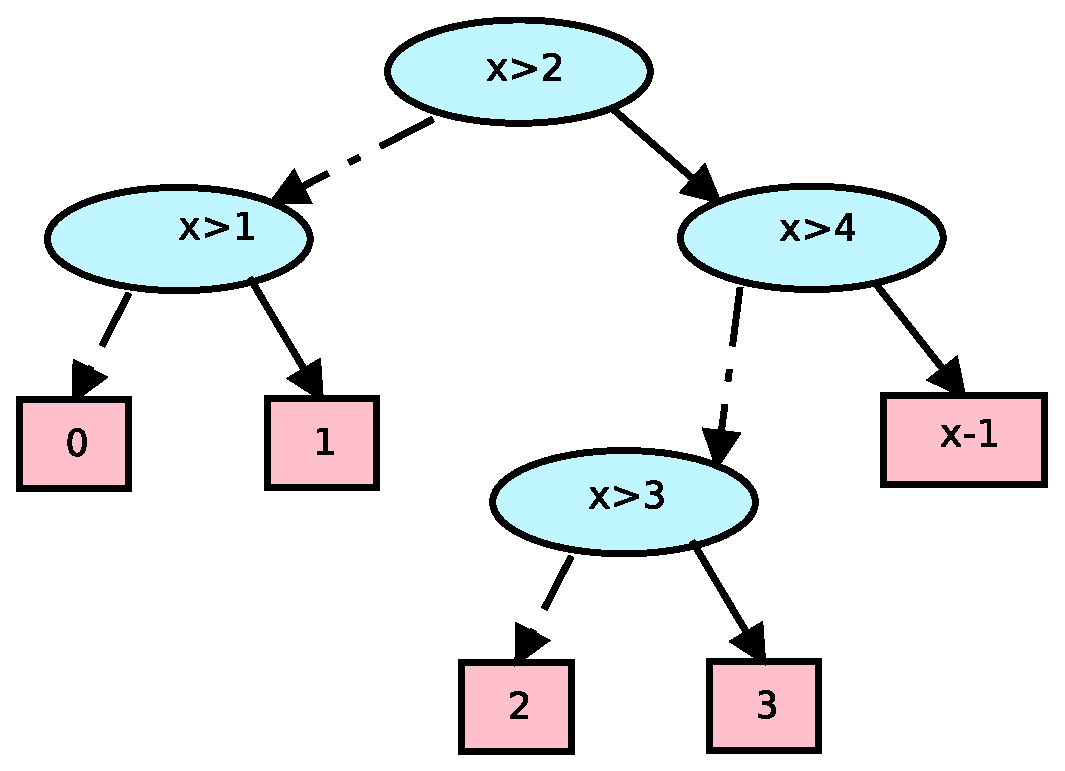
\includegraphics[scale=0.4]{Figures/xadds/samplexadd.eps} }
\caption{ Example of XADD.}
\label{fig:xaddex} 
\end{figure}

Binary operations as addition and multiplication can be performed in XADD analogously  to the ADD version, as the expressions themselves support this operations. The division operation, however, is not closed in polynomial expressions, and thus is not supported in polynomial XADDs. The boolean variable marginalization simply involves an addition so is also supported. Still, unary maximization or minimization involves obtaining extremum from arbitrary polynomials, and thus is only supported in exact form for linear XADDs. An operation that requires detailed description is the binary maximization. It is closed form both in linear and polynomial XADDs, but introduce new decisions. We define \emph{symbolic binary maximization} in the case representation as follows, and illustrate it as an XADD operation in figure~\ref{fig:xaddmax}:

\begin{figure}[h!t]
\center
\fbox{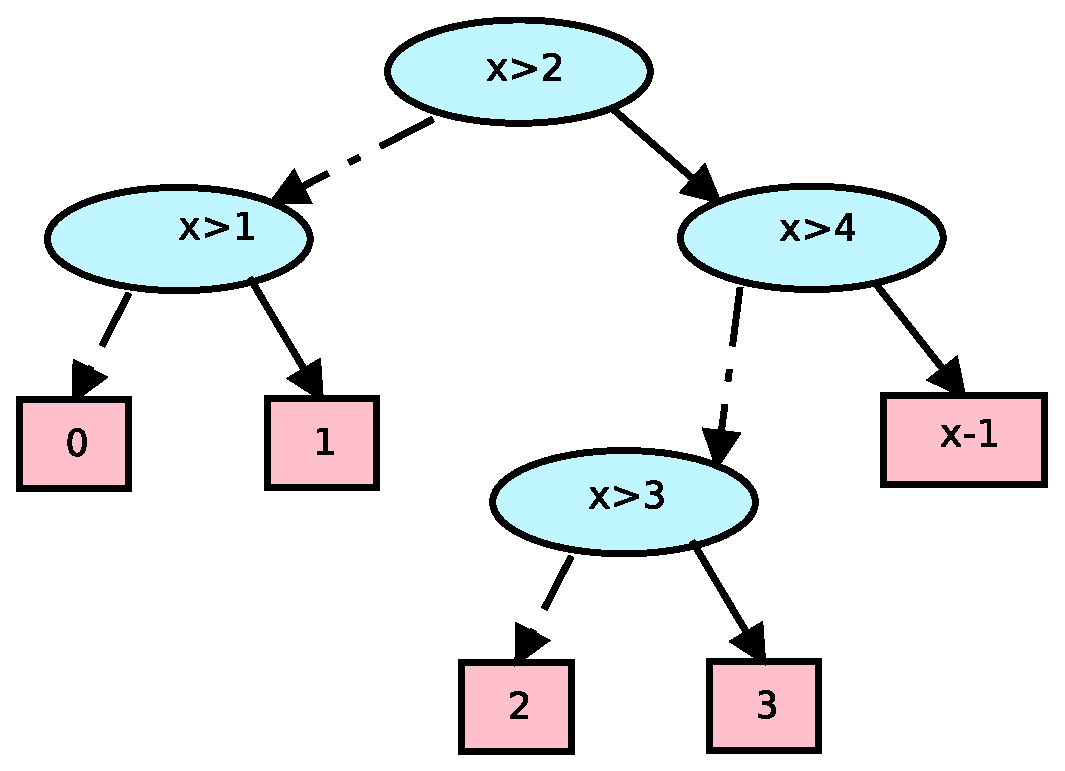
\includegraphics[scale=0.4]{Figures/xadds/samplexadd.eps} }
\caption{ Example of XADD max Operation.}
\label{fig:xaddmax} 
\end{figure}


\vspace{-5mm}
{\footnotesize
\begin{center}
\begin{tabular}{r c c c l}
&
\hspace{-7mm} $\casemax \Bigg(
  \begin{cases}
    \phi_1: \hspace{-2mm} & \hspace{-1mm} f_1 \\ 
    \phi_2: \hspace{-2mm} & \hspace{-1mm} f_2 \\ 
  \end{cases}$
$,$
&
\hspace{-4mm}
  $\begin{cases}
    \psi_1: \hspace{-2mm} & \hspace{-1mm} g_1 \\ 
    \psi_2: \hspace{-2mm} & \hspace{-1mm} g_2 \\ 
  \end{cases} \Bigg)$
&
\hspace{-4mm} 
$ = $
&
\hspace{-4mm}
  $\begin{cases}
  \phi_1 \wedge \psi_1 \wedge f_1 > g_1    : & \hspace{-2mm} f_1 \\ 
  \phi_1 \wedge \psi_1 \wedge f_1 \leq g_1 : & \hspace{-2mm} g_1 \\ 
  \phi_1 \wedge \psi_2 \wedge f_1 > g_2    : & \hspace{-2mm}f_1 \\ 
  \phi_1 \wedge \psi_2 \wedge f_1 \leq g_2 : & \hspace{-2mm} g_2 \\ 
  \hspace{1cm}\vdots \hspace{8mm}: & \hspace{-2mm} \vdots
  \end{cases}$
\end{tabular}
\end{center}
\vspace{-3mm}
} If all $f_i$ and $g_i$ are linear,
the $\casemax$ result is clearly still linear and representable in the case format previously described (i.e., linear inequalities in decisions).

In the rest of the paper, we will consider only linear XADDs, i.e. XADD with only linear expressions on the continuous variables, because linear XADDs permit LP solvers to be used in two ways: linear constraint feasibility checking to prune unreachable paths in the XADD and linear constrained optimization of linear functions to obtain maximum and minimum values of a XADD. Besides, our main contribution in this paper is the development of an bounded error approximation method for piecewise linear functions that is used in linear XADDs to increase efficiency.